\documentclass{whutmod}
\usepackage{metalogo}
\usepackage{float}
\usepackage{subfigure} 
\usepackage{url}
\usepackage{booktabs}
\bibliographystyle{unsrt}
\team{23}
\membera{刘子川}
\joba{编程}
\memberb{程宇}
\jobb{建模}
\memberc{陈荣兴}
\jobc{建模}
\hypersetup{
	colorlinks=true,
	linkcolor=black
}

\title{基于因子分析与灰色关联分析对武汉市人才吸引力的量化评价}
\tihao{4} 

\begin{document}

	%\maketitle
	
	\begin{abstract}

植物的种类繁多,为研究植物分类方法,本文基于植物树叶的二值化图片数据,通过\textbf{解析几何计算}和\textbf{时间序列展开}的方法转换成轮廓特征向量和边缘特征向量;再通过\textbf{粒子群算法}优化的\textbf{深度神经网络}解决树叶识别分类问题,并分析核心指标对模型性能的影响,最终结合树叶纹理信息对模型进行改进和分析比较。
~\\

针对问题一,通过\textbf{解析几何计算}和\textbf{时间序列展开},分别提取每一张图片中的特征向量。根据题目要求,本组首先利用\textbf{matlab}计算与图像形状相关的解析几何特征量,得到由八个几何学、拓扑学特征值组成的\textbf{八维}形状特征向量。然后将图像轮廓进行极化投影,并通过\textbf{numpy工具箱}将极化投影轮廓展开成时间序列,挖掘分析时间序列的三个特征值,组成\textbf{三维}边缘特征向量。最后合并两个向量得到\textbf{十一维}总体特征向量。~\\


针对问题二,基于问题一中提取的特征信息,建立了\textbf{PSO-DNN网络}对树叶进行识别与分类。利用\textbf{Keras工具库}搭建\textbf{深度神经网络},利用\textbf{粒子群算法}优化DNN网络的连接权值和阈值,对研究对象进行识别分类。训练后的神经网络模型预测准确率为$\textbf{91.037\%}$,并分析各指标的权重占比,判断出特征量中\textbf{时间序列熵、密实度和最大压痕深度}对模型性能影响最大,是模型的核心指标。将其剔除后,模型分类精确度损失率分别为\textbf{6.937\%、5.498\%、3.559\%}。
~\\

针对问题三,基于问题二中的\textbf{PSO-DNN网络}模型,将树叶纹理信息嵌入特征向量。增加网络输入层个数,并对模型进行参数调整,最终得到叶片的预测准确率达到$\textbf{96.634\%}$。
~\\

本文中所提到的模型优点主要有两点:一、提取的特征值信息包含量大、区分度高;二、利用PSO优化后的DNN网络全局收敛能力强,分类准确度高。

	
  
\keywords{时间序列展开\quad  深度神经网络\quad  粒子群算法\quad Keras工具库\quad }
		
	\end{abstract}
	
	%目录
	\tableofcontents
	\newpage	%换页符
	
	\section{问题重述}	
	\subsection{问题背景}
    诺曼底登陆:代号“霸王行动”,是第二次世界大战中盟军在欧洲西线战场发起的一场大规模攻势,接近三百万士兵渡过英吉利海峡前往法国诺曼底。诺曼底战役是人类战争史上规模最大的一次海上登陆战役行动,使第二次世界大战的战略态势发生了根本性的变化。
    
    海运装载是海上登陆战役中的一种作战行动,将需要登陆的部队人员、装备、补给品装载到海上运输工具,该行动会直接影响着登陆作战效果。以诺曼底战役的第一批海上登陆输送兵力为参考,不同成建制单位的部队人员、装备和补给品都有不同的数量级需求,研究合理利用海军运输船和民用船只进行兵力装载以及对装载方案的优化都具有重要意义。
    
    
    

	\subsection{问题概述}
    围绕相关附件和条件要求,研究海运装载行动输送兵力任务的合理安排,依次提出以下问题:
		 
	
	\textbf{问题一:}根据输送任务和海上运输工具情况,结合相关条件和要求,分析运输船舰和兵力的关系,概算各类型旅一个旅级单位的运输工具的需求量,并给出具体装载方案。
	
	\textbf{问题二:}根据输送任务,结合附件中的港口及码头泊位,制定时间最短、船只数量最少的兵力装载方案。
	
	\textbf{问题三:}假设装载行动开始24小时后,A港口的两个A1和一个A2泊位,D港口的一个D2和两个D3泊位被毁,给出具体调整方案以及完成装载任务的对策建议。
	
	
	\section{模型假设}
	\begin{itemize}                                             
		\item [(1)] 为了简化计算,假设题目中给出的模糊数据都是精确数据。
		\item [(2)] 为了优化运算结果,假设所有全副武装的士兵都保持坐姿休息。
		\item [(3)] 假设在战争中,装载消耗更少时间的优先度高于使用更少的民用船。
		\item [(4)] 假设在装载过程中,同一泊口的船舰装载交替时间可以忽略不记。
		\item [(5)] 假设港口被摧毁时,由于提前得到信息,港口上的船只与兵力没有损失,只是正在进行的装载工作停止,且进度完全损失。
	\end{itemize}
	
	
	\section{符号说明}
%	每行都有线的表
%	\begin{center}
%		\begin{tabular}{cc}
%			\hline
%			\makebox[0.3\textwidth][c]{符号}	&  \makebox[0.4\textwidth][c]{意义} \\ \hline
%			$C_{0}$	    &  污染源初始浓度 \\ \hline
%			$C(x,t)$	    &  污染浓度随时空变化 \\ \hline
%			$u_{x}$	    &  江河平均纵向流速 \\ \hline
%			$E_{x}$  &  铊在江河纵向弥散系数\\ \hline
%		$p$   &  面污染物纵向距离\\ \hline
%			$K_{c}$	    & 污染物降解系数  \\ \hline
%		    $a$	& 污染超标系数 \\ \hline
%		     $x$	& 距污染源的一维距离 \\ \hline
%		      $t$	& 距污染发生后的时间 \\ \hline
%		       $V_{A}$	& 溶液摩尔体积 \\ \hline
%		      $M_{B}$	& 江水的摩尔质量 \\ \hline
%		     $\mu_{B}$	& 溶剂的粘度 \\ \hline		      
%		\end{tabular}
%	\end{center}

%三线表
	\begin{table}[H]
	\label{biao} \centering
		\begin{tabular}{cc}
			\toprule[1.5pt]
			\multicolumn{1}{m{5cm}}{\centering 符号} & \multicolumn{1}{m{5cm}}{\centering 说明} \\
			\midrule[1pt]
			$I$  &  研究图像 \\ 
			$A(I)$  &  图像面积 \\ 
			$C(I)$  & 图像几何中心\\
			$\partial I$  &  图像边界 \\ 
		    $d(.)$ & 运算两点间欧式距离\\
			$ID$	 &  总特征向量  \\ 
			$ID_{shape}$ &  形状特征向量 \\ 
			$ID_{margin}$	 &  边缘特征向量 \\ 
			$id_{k}$  &   研究图像特征值\\ 
			$r$  &  极径\\	
			$\theta$ & 极角\\
			$X$ &  时间序列集\\ 
			$S$ & shapelet子序列\\
			$x_{i}$ & 神经网络第$i$个输入值\\
			$w_{ki}$ & 第$i$个输入量连接的权值\\
			$b_{k}$ & 神经网络阈值\\
			$f$  & 激活函数\\
			$e$ & 误差函数\\
			$E$ & 全局误差\\
			$\eta $ &  学习率\\
			$c_{1,2}$ & 加速因子\\
			$\beta$ & 惯性权重\\
			

		
			\bottomrule[1.5pt]
		\end{tabular}
	\end{table}

	\section{问题一模型的建立与求解}

    \subsection{问题描述与分析}
    问题一要求根据输送任务和船舰情况,结合相关条件和要求,分析运输船舰和兵力的关系,概算各类型旅一个旅级单位对船舰的需求量,给出装载方案。其本质是一个多背包优化问题,要求使用尽可能少的背包,装载各种旅的一个旅编制兵力。本组首先对兵力、装备与装载的面积进行量化,根据题目要求,以派出船舰种类和数量作为决策向量,以所用的总船只数量为目标函数,设计沙石算法,使得每艘船面积利用率达到最高,从而使得调用船支数达到最小值。
    

	    \subsection{模型的建立}
	    \subsubsection{预备工作}
	    \paragraph{兵力、装备与船载的面积量化}
	    计算附件2中的每种装备与所占面积:
	    \begin{gather}
	    s_{xi}=l_{i}\times w_{i} \times \varepsilon _{i}
	    \end{gather}
	    其中$s_{xi}$是装备$X_{i}(i=1,2\cdots,14)$的占用面积,$l_{i}$、$w_{i}$与$\varepsilon _{i}$分别是装备$X_{i}$的长、宽与面积修正系数。得到装备占用面积向量:
	     \begin{gather}
	     S_{x}=[s_{x1},s_{x2},\cdots,s_{x14}]
	     \end{gather}
	     计算附件2中每种旅一个营的占用面积:
	     \begin{gather}
	     s_{pi}=p_{i}\times s
	     \end{gather}
	     其中$p_{i}$是第$i(i=1,2,\cdots,12)$的全副武装人员数,取$s=0.5m^2$为每个全副武装人员占用的面积。得到每营人口所占面积向量:
	     \begin{gather}
	     S_{p}=[s_{p1},s_{p2},\cdots,s_{p12}]
	     \end{gather}
	     计算附件3中船舰可用装载面积:
	      \begin{gather}
	      s_{yi}=s_{i}\times \eta_{1}
	      \end{gather}
	    其中$s_{yi}$是登陆舰$Y_{i}(i=1,2\cdots,14)$的可用装载面积,$s_{i}$是登陆舰$Y_{i}$的总装载面积,取$\eta_{1}=75\%$为登陆舰的有效面积率。得到登陆舰有效面积向量:
	     \begin{gather}
	     S_{y}=[s_{y1},s_{y2},\cdots,s_{y14}]
	      \end{gather}
	      \begin{gather}
	      s_{zj}=s_{j}\times \eta_{2}
	      \end{gather}
	       其中$s_{zi}$民用船$Z_{j}(i=1,2\cdots,5)$的可用装载面积,$s_{j}$是民用船$Z_{j}$的总装载面积,取$\eta_{2}=70\%$为登陆舰的有效面积率。得到登陆舰有效面积向量:
	       \begin{gather}
	       S_{z}=[s_{z1},s_{z2},\cdots,s_{z5}]
	      \end{gather}

	    \subsubsection{优化函数与约束条件}
	    \textbf{决策向量}为:
	     \begin{gather}
	     D=[y_{1},y_{2},\cdots,y_{14},z_{1},z_{2},\cdots,z_{5}]
	    \end{gather}
	    其中$y_{k}$是派出的登陆舰数量,$z_{k}$是派出民用船的数量。
	    
	    根据题意尽可能使用少的船舰数,即\textbf{目标函数}为使用船舰总数:
	     \begin{gather}
	     min Z=\sum D
	  \end{gather}
	    
	    
	   舰载面积系数向量为:
	    \begin{gather}
	    S_{D}=[S_{y}, S_{z}]
    	\end{gather}
    	根据题目要求总舰载有效面积不小于总兵力装备占用面积:
    	 \begin{gather}
    	 D\cdot S_{D}\geq \sum  S_{x} + \sum  S_{p}
    	 \end{gather}
    	 且由登陆舰Y1的有效舰载面积大于装备X9(直升机)的部队占用的面积:
    	  \begin{gather}
    	 y_{1}\cdot s_{y1}\geq \sum s_{x9}+ \sum  s_{p6}
    	 \end{gather}
    	 其中$\sum  s_{p6}$是唯一装备的部队——$\uppercase\expandafter{\romannumeral6}$旅的人口总和。
    	 

    	 建立得到使用最少船舰装载每种旅各一个旅级编制的模型为:
    	  \begin{gather}
    	 min Z=\sum D\\ 
    	  s.t.\left\{\begin{matrix}	 D\cdot S_{D}\geq \sum  S_{x} + \sum  S_{p}
    	 \\ y_{1}\cdot s_{y1}\geq \sum s_{x9}+ \sum  s_{p6}
    	 \\S_{D}=[S_{y}, S_{z}]
    	 \\ s_{xi}=l_{i}\times w_{i} \times \varepsilon _{i}
    	 \\S_{x}=[s_{x1},s_{x2},\cdots,s_{x14}]
    	 \\s_{pi}=p_{i}\times s
    	 \\S_{p}=[s_{p1},s_{p2},\cdots,s_{p12}]
    	 \\     s_{yi}=s_{i}\times \eta_{1}
    	 \\   S_{y}=[s_{y1},s_{y2},\cdots,s_{y14}]
    	 \\      s_{zj}=s_{j}\times \eta_{2}
    	 \\ S_{z}=[s_{z1},s_{z2},\cdots,s_{z5}]
    	 \end{matrix}\right. 
     	 \end{gather}

    		    	
	\subsection{模型的求解}
  
	     
	     %其算法流程图如图~\ref{77}~

	      %\begin{figure}[H]
	      %	\centering
	      %	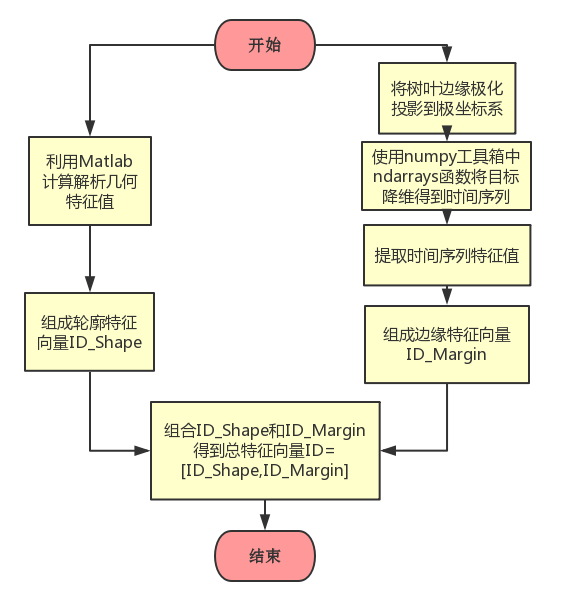
\includegraphics[width=.8\textwidth]{figures/lct.png}
	      %	\caption{树叶特征工程示意图}\label{77}
	      %\end{figure}
		
    	  \subsubsection{沙石算法}
		为使得调用的船舰数量最少,即需使得每艘船的未利用面积值达到最小:
	    \begin{gather*}
		min \Delta S= \sum  S_{x} + \sum  S_{p}-D\cdot S_{D} 
		\end{gather*}
	其中$\Delta S$为损失面积,本组设计沙石算法优化部队装载方案,使其得面积损失达到最小,具体如下:
	 \paragraph{算法思想}
	 根据经验,使用沙砾和石子填满某个刚性容器,较好的方法是先装入石子,后灌入沙砾,可以让剩余空间达到最小。基于此,本组设计沙石算法,将带待装载部队(其占用面积不尽相同)视作沙砾与石子,将船舰视作刚性容器,即可求出面积利用率最高的部队装载方案。沙石算法示意图如图 ~\ref{shashi}~所示:
	 
	 
	 \begin{figure}[H]
	 	\centering
	 	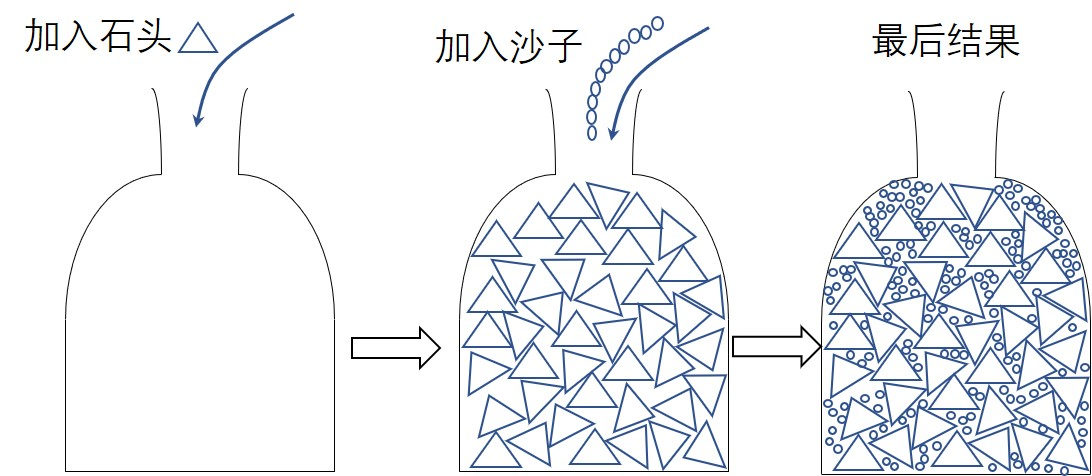
\includegraphics[width=.8\textwidth]{figures/shashi.jpg}
	 	\caption{沙石算法示意图}\label{shashi}
	 \end{figure}
	 
	 \paragraph{算法描述}
	 	\begin{itemize}
	 	\item [(1)] 装备均分:将每个旅分解为连编制,即得到面积规划向量:
	 \begin{gather*}
	 	A^k=[a^k_{1},a^k_{2},\cdots,a^k_{n}]
	\end{gather*}
	 	其中$a^k_{i}$的初始值是第$k$旅中的全副武装人员所占面积,其中$k=1,2,\cdots,K$($K$为旅队编制总数),$n=n_{k}$($n_{k}$为k旅连编制总数)。根据题目中装备均匀分配的要求,重复检索向量$A^k$中的每一个元素,选择最小值$min \left \{ a_{i} \right \}$ (装备量最少的营)使得该连添加装备$X_{j}$,即令:
	 	\begin{gather*}
	   min \left \{ a_{i} \right \}=min \left \{ a_{i} \right \}+s_{xj}
	 	\end{gather*}
	 	重复检索直到该旅装备数$X=0$时,结束装备均分,得到装备均分后的部队$ \left \{A^k\right \}(k=1,2,\cdots,n_{k})$($n_{k}$为k旅连编制总数)。
	
		\item [(2)] 部队装载:将装备均分后的部队$ \left \{A^k\right \}$中的元素混合后由大到小进行排序得到排序后的营编制总部对数列$ \left \{T_{n}\right \}$:
			\begin{gather*}
	T_{n}\geqslant 	T_{n+1}\\
	n\leq \sum_{1}^{K}n_{k}
		\end{gather*}
		将所有派出船舰装载面积进行排序得到船舰面积数列$ \left \{P_{n}\right \}$:
	
		依次检索总部对数列$ \left \{T_{n}\right \}$,并依次检索数列$ \left \{P_{n}\right \}$对应的船舰,将其装入剩余面积足够的船舰,即若$P_{n}\geqslant T_{n}$ 令:
		\begin{gather*}
		P_{n}=	P_{n}-	T_{n}
		\end{gather*}
		重复检索直到部队装载完成,即当部队检索次数$i=\sum_{1}^{K}n_{k}$时,算法结束。

		\item [(3)] 结果输出:输出总共使用的船舰编号,即决策向量:
		\begin{gather}
		D=[y_{1},y_{2},\cdots,y_{14},z_{1},z_{2},\cdots,z_{5}]
		\end{gather}
	\end{itemize}      	
	
	
	\subsection{结果分析}

		\begin{table}[H]
		\centering		\caption{各旅级单位装备人口面积装载方案}\label{zhuangzai}
		\begin{tabular}{cccccc}
			\toprule[2pt]
			\multicolumn{1}{m{2cm}}{\centering 船舰类别}
			& \multicolumn{1}{m{2cm}}{\centering 第Ⅰ型旅}
			&\multicolumn{1}{m{2cm}}{\centering 第Ⅱ型旅}
			& \multicolumn{1}{m{3cm}}{\centering $ \cdots \cdots  $}
			& \multicolumn{1}{m{2cm}}{\centering 第Ⅺ型旅}
			& \multicolumn{1}{m{2cm}}{\centering 第Ⅻ型支队(旅)}
			\\
			\midrule[1pt]
			Y1综合登陆舰 &  $267.6285185$  &$0$ & $\cdots \cdots$&$5658.770914
			$ &$42.85714286$ \\ 
			Y2大型登陆舰	 &  $1586.951111$&$0$& $\cdots \cdots$ &$0$ &$0$\\ 
			Y3大型登陆舰	 &  $3178.042222 $ &$0$& $\cdots \cdots$ &$5864.014286
			$ &$0$\\ 
			Y4大型登陆舰	 &  $2114.508148 $ &$0$& $\cdots \cdots$ &$0
			$ &$0$\\ `
			$\cdots \cdots$	 &  $\cdots \cdots$  &$\cdots \cdots$ &$\cdots \cdots$ &$\cdots \cdots$ &$\cdots \cdots$\\ 
			Y12登陆艇	 &  $0$ &$0$ & $\cdots \cdots$ &$0$ &$728.5714286$\\ 
			Y13登陆艇	 &  $0$ &$0$ & $\cdots \cdots$ &$0$ &$0$\\ 
			Y14登陆艇		 &  $0$ &$0$ & $\cdots \cdots$ &$0$ &$0$\\ 
			2万吨级滚装船  &  $0 $ &$6549.897037$& $\cdots \cdots$ &$0$ &$0$ \\ 
			\bottomrule[2pt]	
		\end{tabular}
	\end{table}

	

		
	\section{问题二模型的建立与求解}
	\subsection{问题的描述与分析}
	问题二要求针对附件2中的具体运输任务,制定使得装载时间最短,使用海上运输工具最少的兵力装载方案。本组通过遗传算法,将问题一中的决策向量作为染色体,装载时间和船支数量作为适应度函数,建立装载方案优化模型。首先修改问题一中的沙石算法,作为判断每个个体是否可以存活的基础。并生成$w$个初始个体
	

		
	\begin{figure}[H]
	\centering
	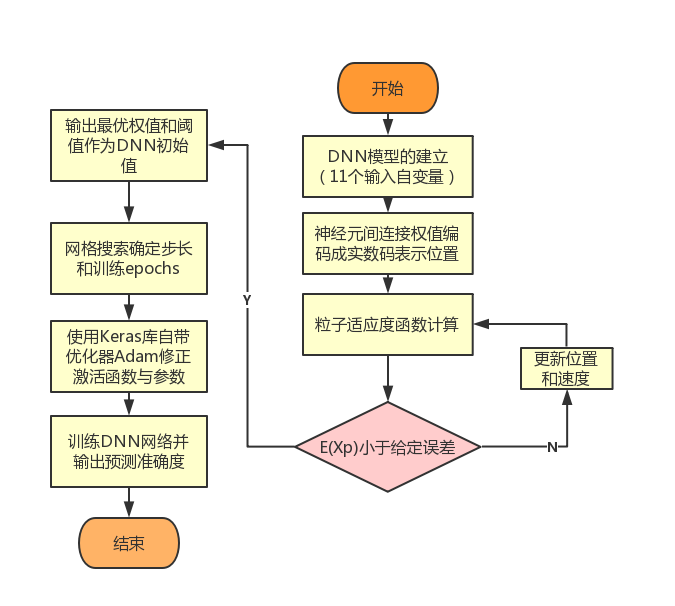
\includegraphics[width=\textwidth]{figures/21.png}
	\caption{PSO算法优化DNN网络流程图}\label{2222}
	\end{figure}


	\subsection{模型的建立与求解}
	
	\subsubsection{DNN网络搭建}
	DNN的正向传播主要依靠众多神经元的计算来完成的,此处设计的网络结构如图~\ref{dnn}~所示,工作过程中可以用下式来表示:
			\begin{gather}
{u_{k}=\sum_{i=1} w_{k i} x_{i}} \\ {y_{k}=f\left(u_{k}-b_{k}\right)}
	\end{gather}
	其中:$x_{i}$表示第 i 个输入; $w_{ki}$表示与第 i 输入量相 连的权值; $u_{k}$表示所有输入的加权和; $b_{k}$为神经 元阈值;$ f$ 为激活函数; $y_{k}$ 为神经网络的输出。
	
	激活函数的种类有很多,如 $sigmoid$, $tanh$ 及$ Relu$,本文应用的是 $Relu$作为激活函数搭建两层隐含层,如式~\ref{shiw}~所示:
	\begin{gather}\label{shiw}
		\begin{array}{c}{f_{\text {Relu}}=\max (0, z)}\\
		\frac{d}{d z} f_{R e L U}=\left\{\begin{array}{ll}{1,} & {z>0} \\ {0,} & {z \leqslant 0}\end{array}\right.
		\end{array}
	\end{gather}
	
	网络的输出层使用$ softmax $函数作分类器, 式~\ref{shiq}~为第 i 个神经的输出:
	\begin{gather}\label{shiq}
		f_{\text {softinax }}=\mathrm{e}^{i} / \sum_{j} \mathrm{e}^{j}
	\end{gather}
	具体算法步骤如下:
	\begin{itemize}
	\item [(1)]进行网络的初始化设置,用$(-1,1)$之间的随机数对DNN各个层的权值和阈值分别进行相应初始化,设定误差函数为$e$、计算精度为$\epsilon $、学习速率为$\eta $以及最大学习次数为$M$。

	\item [(2)]随机选取第$k$次输入样本$x(k)$以及对应的实际期望输出$d(k)$如下:
	\begin{gather*}
	x(k)=[x_{1}(k),x_{2}(k),...,x_{n}(k)]\\
	d(k)=[d_{1}(k),d_{2}(k),...,d_{r}(k)]
	\end{gather*}
	
	\item [(3)]计算DNN中第$1$隐含层、第$2$隐含层以及输出层的输入值和输出值具体计算公式如下:

	\begin{gather*}
	h_{\mathrm{bs}} (k)=\sum_{i=1}^{n} u_{i s} x_{i}(k)+b_{s} \quad s=1,2, \cdots,p\\
	h_{\mathrm{os}} s(k)=f_{1}\left(h_{\mathrm{bs}}(k)\right) \quad s=1,2, \cdots, p	\\
    g_{\mathrm{bt}}(k)=\sum_{s=1}^{p} v_{s t} h_{\mathrm{os}}(k)+b_{t} \quad t=1,2, \cdots, q\\
   	g_{\mathrm{ot}}(k)=f_{2}\left(g_{\mathrm{bt}}(k)\right) \quad s=1,2, \cdots, q	\\
   	y_{\mathrm{bj}}( k )=\sum_{i = 1 }^{q}w_{ij}g_{\mathrm{at}}(k)+b_{j} \quad j = 1,2 , \cdots,r\\
   y_{\mathrm{oj}}( k ) = f _ { 3 } \left( y _ { b j } ( k ) \right) \quad j = 1,2 , \cdots,r
	\end{gather*}
	其中$x_{i}$输入层输入向量,$h_{\mathrm{b}}$为第$1$隐含层输入向量,$h_{\mathrm{o}}$为第$1$隐含层输出向量,$g_{\mathrm{b}}$为第$2$隐含层输入向量,$g_{\mathrm{o}}$为第$2$隐含层输出向量,$y_{\mathrm{b}}$为输出层输入向量,$y_{\mathrm{o}}$为输出层输出向量
	输入向量
	\item [(4)]首先给定误差函数如下:
	\begin{gather*}
	e = \frac { 1 } { 2 } \sum _ { j = 1 } ^ { r } \left( d _ { j } ( k ) - y _ { bj } ( k ) \right) ^ { 2 }
	\end{gather*}
	误差函数$e$对输出各层求偏导数得:
		\begin{gather*}
        \frac { \partial e } { \partial y _ { b j}(k) }=\delta _{j}(k)\\
        \frac { \partial e } { \partial g _ { bt }(k) }=\delta _{t}(k)\\
        \frac { \partial e } { \partial h _ { bs} }(k)=\delta _{s}(k)
        \end{gather*}

	即通过$\delta$值与各层的输出修正各层级间的权值,其计算公式如下:
	\begin{gather*}
	w _ { t j } ^ { N + 1 } = w _ { t j } ^ { N } + \eta \delta _ { j } ( k ) g _ { o t } ( k )\\
	w _ { s t } ^ { N + 1 } = w _ { s t } ^ { N } + \eta \delta _ { t } ( k ) g _ { o s } ( k )\\
	w _ { i s } ^ { N + 1 } = w _ { i s } ^ { N } + \eta \delta _ { j } ( k ) g _ { o t } ( k )
	\end{gather*}
	同理,各层级阈值变化公式如下
	\begin{gather*}
	\begin{array} { l } { \Delta b _ { j } ( k ) = \eta \delta _ { j } ( k ) } \\ { \Delta b _ { l } ( k ) = \eta \delta _ { t } ( k ) } \\ { \Delta b _ { s } ( k ) = \eta \delta _ { s } ( k ) } \end{array}
	\end{gather*}
	使用当前权值计算全局误差,公式如下:
	\begin{gather*}
	E = \frac { 1 } { 2 m } \sum _ { k = 1 } ^ { m } \sum _ { j = 1 } ^ { r } \left( d _ { j } ( k ) - y _ { o j } ( k ) \right) ^ { 2 }
	\end{gather*}
	当误差小于预设精度$\varepsilon $或达到最大学习次数$M$时网络算法结束,否则返回(2)进行下一轮学习训练.
		\end{itemize}
	
		\begin{figure}[H]
		\centering
		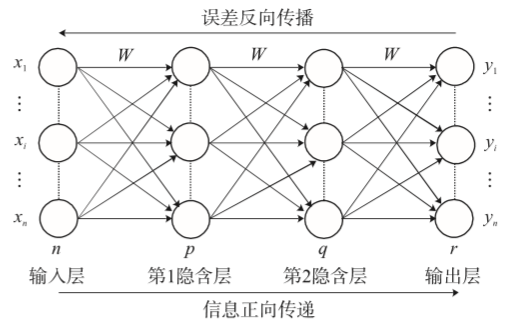
\includegraphics[width=\textwidth]{figures/123546.png}
		\caption{人工搭建DNN结构示意图}\label{dnn}
	\end{figure}
	
	
	\subsubsection{PSO优化DNN网络}
	算法的具体实现步骤如下:
	\begin{itemize}
		\item [(1)]将DNN网络结构中所有神经元间的连接权值和各个神经元的阈值编码成实数码串表示的个体作为PSO算法要寻优的位置向量。
		\item [(2)]在编码空间中随机生成一定数目的个体组成种群,其不同个体代表神经网络不同权值。
		\item [(3)]DNN网络训练及个体的适应度评价。将微粒群中的每一个个体的分量映射为网络中的权值和阈值,从而构成个体对应的神经网络。首先划分训练样本和测试样本;其次输入训练样本进行网络训练,通过反复迭代来优化网络权值,并计算每一个网络在训练集上产生的均方误差,,以此作为目标函数;最后对每个个体进行适应度评价,从中找到最佳个体用来判断是否需要更新微粒的Gbest与Pbest,以全局误差值作为适应度函数:
		\begin{gather*}
		E = \frac { 1 } { 2 m } \sum _ { k = 1 } ^ { m } \sum _ { j = 1 } ^ { r } \left( d _ { j } ( k ) - y _ { o j } ( k ) \right) ^ { 2 }
		\end{gather*}
		
		式中:$m$为训练样本个数,
		$r$为输出端个数,$y_{oj}(k)$为训练样本在输出端的给定输出,$ d _ { j } ( k ) $为训练样本在输出端的实测值,他们俩个值的误差平方和越小,表示实际值和预测值越接近,网络的性能越好。
		
		\item [(4)]更新每个粒子的速度和位置,产生下一代的粒子群。更新公式如下:
		\begin{gather}
		v_{id}^{t+1}=v_{id}^{t}+c_{1}r_{1}(p_{id}^{t}-x_{id}^{t})+c_{2}r_{2}(g_{id}^{t}-x_{id}^{t})
		\end{gather}	
		\begin{gather}
		x_{id}^{t+1}=x_{id}^{t}+v_{id}^{t+1}
		\end{gather}
		其中$i=1,2,...,n$;$d=1,2,...,d$;$t$为当前迭代次数;$v_{id}^{t}$为当前粒子速度($t$时刻);$x_{id}^{t}$为当前粒子位置($t$时刻);$(p_{id}^{t}-x_{id}^{t})$为当前位置与自己最好位置之间的距离;$(g_{id}^{t}-x_{id}^{t})$为当前位置与群体最好位置之间的距离;$v_{id}^{t+1}$为下一时刻粒子速度($t+1$时刻);$c_{1},c_{2}$为非负常数,称为加速因子;$r_{1},r_{2}$为均匀分布与$[0,1]$区间的随机数。
		
		\item [(5)]当目标函数小于给定的误差或达到最大迭代次数时,算法结束。将PSO算法训练出来的最佳神经网络的权值和阈值作为DNN网络的初始值,并记录计算指标重要度:
		\begin{gather}
			Ipot(k)=\sum \left |  w _ { t j }(k)\right |
		\end{gather}
	其中$w _ { t j }(k)$为特征值$id_{k}$训练后的输入权重。
	\end{itemize}
	
	\subsubsection{参数的选取与确定}
	由于训练epochs与步长选取较为困难,实验采取\textbf{网格搜索法}(Grid Search)来确定参数的选取,网格搜索是指定参数值的一种穷举搜索方法,通过将估计函数的参数通过交叉验证的方法进行优化来得到最优的学习算法。
	
	在迭代修正的过程中,实验采用$Keras$自带优化器\textbf{Adam函数}进行迭代修正,如式~\ref{adam}~所示,其中$\beta_{1}$一般取0.9,$\beta_{2}$一般取0.999。
	
	\begin{gather*}\label{adam}
	\left\{\begin{array}{l}{m_{t}=\beta_{1} m_{t-1}+\left(1-\beta_{1}\right) \nabla_{w} f\left(w_{t}\right)} \\ {v_{t}=\beta_{2} v_{t-1}+\left(1-\beta_{2}\right) \nabla_{w} f\left(w_{t}\right)^{2}} \\ {\widehat{m}_{t}=\frac{m_{t}}{1-\beta_{1}^{t}}, \hat{v}_{t}=\frac{v_{t}}{1-\beta_{2}^{t}}} \\ {w_{t}=w_{t-1}-\eta \frac{\widehat{m}_{t}}{\sqrt{\hat{v}_{t}+\varepsilon}}}\end{array}\right.
	\end{gather*}


	\subsection{实验与结果分析}
	随机选取80\%的数据作为训练集进行数据\textbf{标准化处理},再对树叶种类(species)进行\textbf{One-Hot编码}作为分类目标。训练输入样本为$1280*11$,测试输入样本为$320*11$,DNN网络输入层神经元$11$个,输出层神经元$100$ 个,包含$2$个隐含层,适应度函数选择均方误差。按照PSO优化DNN网络模型的步骤不断地迭代寻找最优网络参数,进行树叶分类预测的仿真实验。具体参数设置间表~\ref{canshu}~。
			\begin{table}[H]
		\centering		\caption{各旅级单位装载方案}\label{zhuangzai}
		\begin{tabular}{cccccc}
			\toprule[2pt]
			\multicolumn{1}{m{3cm}}{\centering 船舰类别}
			& \multicolumn{1}{m{2cm}}{\centering 第Ⅰ型旅}
			&\multicolumn{1}{m{2cm}}{\centering 第Ⅱ型旅}
			& \multicolumn{1}{m{3cm}}{\centering $ \cdots \cdots  $}
			& \multicolumn{1}{m{2cm}}{\centering 第Ⅺ型旅}
			& \multicolumn{1}{m{2cm}}{\centering 第Ⅻ型支队(旅)}
			\\
			\midrule[1pt]
			Y1综合登陆舰 &  $267.6285185$  &$0$ & $\cdots \cdots$&$5658.770914
			$ &$42.85714286$ \\ 
			Y2大型登陆舰	 &  $1586.951111$&$0$& $\cdots \cdots$ &$0$ &$0$\\ 
			Y3大型登陆舰	 &  $3178.042222 $ &$0$& $\cdots \cdots$ &$5864.014286
			$ &$0$\\ 
			$\cdots \cdots$	 &  $\cdots \cdots$  &$\cdots \cdots$ &$\cdots \cdots$ &$\cdots \cdots$ &$\cdots \cdots$\\ 
			Y12登陆艇	 &  $0$ &$0$ & $\cdots \cdots$ &$0$ &$728.5714286$\\ 
			Y13登陆艇	 &  $0$ &$0$ & $\cdots \cdots$ &$0$ &$0$\\ 
			Y14登陆艇		 &  $0$ &$0$ & $\cdots \cdots$ &$0$ &$0$\\ 
			2万吨级滚装船  &  $0 $ &$6549.897037$& $\cdots \cdots$ &$0$ &$0$ \\ 
			\bottomrule[2pt]	
		\end{tabular}

	\end{table}
	
	通过上述参数设置,计算训练后各指标指标重要度,将指标重要度求和,计算每个指标重要度占权得到~\ref{quanzhong}~,最小均方误差为0.458,\textbf{预测准确率为$91.037\%$}。
	其迭代过程中损失与准确率如下图所示:
	\begin{figure}[H]
		\centering
		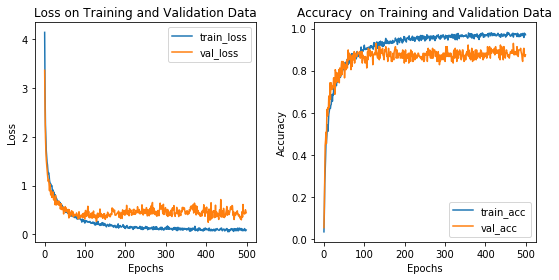
\includegraphics[width=\textwidth]{figures/x.png}
		\caption{PSO-DNN迭代过程中损失与准确率}\label{xxx}
	\end{figure}

	\begin{figure}[H]
	\centering
	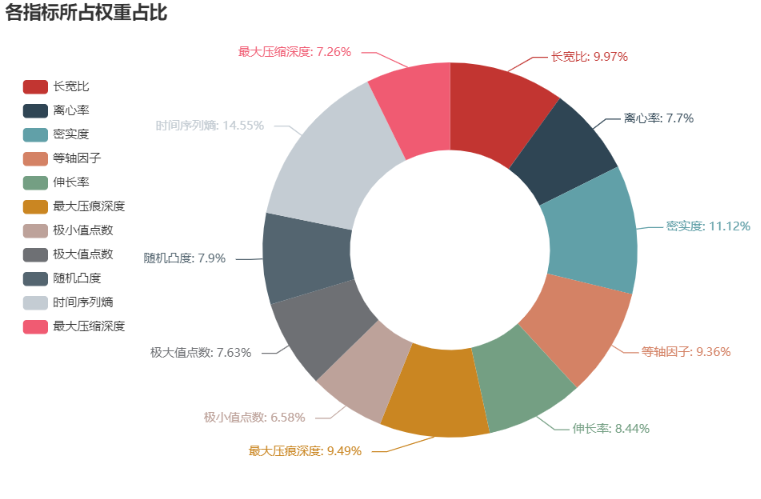
\includegraphics[width=\textwidth]{figures/quanzhong2.png}
	\caption{指标重要度占权图}\label{quanzhong}
		
\end{figure}

	由图~\ref{quanzhong}~可知各指标对模型判别性能的影响,选取重要度占比最高的三个指标——时间序列熵,密实度,最大压痕深度作为核心指标。分别剔除三个指标,再次进行训练与预测,得到缺失核心指标的模型性能如下:
	
		\begin{table}[H]
		\centering	\caption{缺失核心指标的模型性能}\label{hengl}
		\begin{tabular}{ccc}
			\toprule[2pt]
			\multicolumn{1}{m{3cm}}{\centering 缺失指标}
			& \multicolumn{1}{m{3cm}}{\centering 分类准确度}
			&\multicolumn{1}{m{3cm}}{\centering 精度损失率}
			\\
			\midrule[1pt]
			时间序列熵	 & 84.721\%  &6.937\%  \\ 
			密实度	 &  86.112\% &5.498\%  \\ 
			最大压痕深度	 &  87.538\% &  3.559\%  \\ 
		
			\bottomrule[2pt]	
		\end{tabular}
		
	\end{table}

%	从图~\ref{xxx}~可以看出,PSO-DNN网络训练后,在测试集中表现良好效果良好,在
	\subsubsection{模型性能评估}
	表~\ref{heng}~中,实验与三种神经网络进行纵向比较可知,四种神经网络训练后准确率都在90\%左右,证实了神经网络非线性映射能力较强。Elman网络和DNN网络的测试准确率都大于BP网络,说明反馈动态网络的逼近能力要强于前反馈静态网络。使用PSO优化DNN网络后,模型的跟踪性能有所改善,测试集中损失(Validation Loss)仅为0.458,说明PSO-DNN网络的泛化能力和稳定性明显提高,且全局收敛性增强。
	
		\begin{table}[H]
	 \centering	\caption{常见神经网络的比较}\label{heng}
		\begin{tabular}{ccc}
			\toprule[2pt]
			\multicolumn{1}{m{3cm}}{\centering 网络类型}
			 & \multicolumn{1}{m{3cm}}{\centering 网络名称}
			  &\multicolumn{1}{m{4cm}}{\centering 测试集中准确率}
			  \\
			\midrule[1pt]
			静态网络	 &  BP &87.424\%  \\ 
			静态网络	 &  Elman &90.541\%  \\ 
			动态网络	 &  DNN &89.912\%  \\ 
			动态网络	 &  PSO-DNN &91.037\%  \\ 
			\bottomrule[2pt]	
		\end{tabular}

	\end{table}



	\section{问题三模型的建立与求解}
    \subsection{问题描述与分析}
    针对问题三,本题要求结合给出的叶子纹理的数据信息,对问题二原有模型进行改进并进行分析比较。本组基于问题二模型中原有的11维数据,加入叶子纹理的数据信息后增加网络输入层个数,修改PSO-DNN网络的参数,从而提高了叶片识别与分类的精度。
		
    \subsection{模型的建立与求解}
    加入叶片纹理数据后,根据第二问中模型原理进行参数调整,进行树叶分类预测的仿真实验:随机选取80\%的数据作为训练集进行数据\textbf{标准化处理},再对树叶种类进行\textbf{One-Hot编码}作为分类目标。训练输入样本为$1280*75$,测试输入样本为$320*75$,DNN网络输入层神经元$75$个,输出层神经元$100$ 个,包含$2$个隐含层,适应度函数选择均方误差。具体参数设置间表~\ref{canshu2}~。具体参数:
    \begin{table}[H]
    	\centering		\caption{参数设置表}\label{canshu2}
    	\begin{tabular}{ccc}
    		\toprule[2pt]
    		\multicolumn{1}{m{4cm}}{\centering 参数名称}
    		& \multicolumn{1}{m{3cm}}{\centering 参数符号}
    		&\multicolumn{1}{m{3cm}}{\centering 参数值}
    		\\
    		\midrule[1pt]
    		选择粒子个数为	 &  T &$30$ \\ 
    		计算精度	 &  $\varepsilon$&$0.00001$  \\ 
    		学习率	 &  $\eta $ &0.01 \\ 
    		最大迭代次数	 &  $M$ &500\\ 
    		维度	 &  $S$ &75 \\ 
    		加速因子1	 &  $c_{1}$ &1.49\\ 
    		加速因子2	 &  $c_{2}$ &1.49 \\ 
    		惯性权重	 &  $\beta $ &$0.9$ \\ 
    		\bottomrule[2pt]	
    	\end{tabular}
        \end{table}
    
    
    通过上述参数设置,训练后求得最小均方误差为$0.253$,\textbf{预测准确率为$96.634\%$},其迭代过程中损失与准确率如下图所示:
    \begin{figure}[H]
    	\centering
    	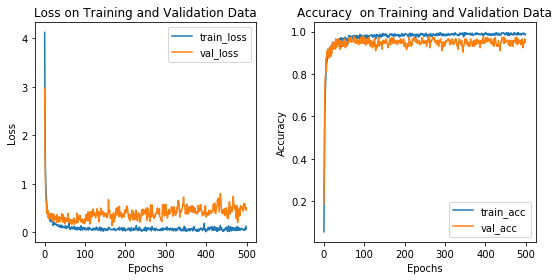
\includegraphics[width=\textwidth]{figures/moxingsan.png}
    	\caption{PSO-DNN迭代过程中损失与准确率}\label{xxxx}
    \end{figure}	
    

    \subsection{结果分析}
	分别与问题二中的PSO优化前后DNN模型进行比较,其结果如下所示:
	\begin{table}[H]
		\centering	\caption{新旧PSO-DNN网络的比较}\label{hengs}
		\begin{tabular}{ccc}
			\toprule[2pt]
						\multicolumn{1}{m{3cm}}{\centering 网络模型}
						&
			\multicolumn{1}{m{3cm}}{\centering Validation Loss}
			& \multicolumn{1}{m{4cm}}{\centering Validation Accuracy}


			\\
			\midrule[1pt]
			新PSO-DNN网络	 &  0.253 &96.634\%  \\ 
			旧PSO-DNN网络	 &  0.458 &91.037\%  \\ 
			新DNN网络	 &  0.291 &95.142\%  \\ 
			旧DNN网络	 &  0.518 &89.912\%  \\ 
			\bottomrule[2pt]	
		\end{tabular}
		
	\end{table}

	结果表明,问题三的PSO-DNN网络在测试集中准确率高于问题二中网络,说明在加入叶子纹理数据后,其分类模型预测能力升高,符合实际情况。与未经过PSO优化权值的网络比较均提升1\%左右,证实了PSO-DNN网络非线性映射能力较强。
	
	\section{模型的评价}
	\subsection{模型的优点}
		\begin{itemize}                                             
		\item [(1)] 利用时间序列提取树叶边缘信息,相较于传统特征量能更准确直观的表述边缘特征。
		\item [(2)] PSO优化后的DNN网络非线性映射能力强,泛化能力和稳定性明显高于一般神经网络,具有更强的鲁棒性。其全局收敛能力强,预测准确度高。
	
	\end{itemize}
	\subsection{模型的缺点}
	树叶二值化图片信息提取不够完全,若能提取更高维度特征向量,分类准确度可进一步提高。

    
	\newpage	%换页符
	%%参考文献
	%\begin{thebibliography}{9}%宽度9
	% \setlength{\itemsep}{-2mm}
	\nocite{*}		%排版未引用的参考文献
%\bibliography{wenxian.bib}
%	%参考文献添加到wenxian.bib里,再引用
%	
\begin{thebibliography}{9}%宽度9
	\bibitem{bib:one} Tan Jing Wei,Chang Siow-Wee,Binti Abdul Kareem Sameem,Yap Hwa Jen,Yong Kien-Thai. Deep Learning for Plant Species Classification using Leaf Vein Morphometric.[J]. IEEE/ACM transactions on computational biology and bioinformatics,2018.
	\bibitem{bib:two}Liu Jing,Sun Wanning,Su Yuting,Jing Peiguang,Yang Xiaokang. BE-CALF: Bit-Depth Enhancement by Concatenating All Level Features of DNN.[J]. IEEE transactions on image processing : a publication of the IEEE Signal Processing Society,2019,28(10).
	\bibitem{bib:three}Matheus B. Vicari,Mathias Disney,Phil Wilkes,Andrew Burt,Kim Calders,William Woodgate. Leaf and wood classification framework for terrestrial LiDAR point clouds[J]. Methods in Ecology and Evolution,2019,10(5).
	\bibitem{bib:}田德红,何建敏.基于变异粒子群优化与深度神经网络的航空弹药消耗预测模型[J].南京理工大学学报,2018,42(06).
	\bibitem{bib:}原继东,王志海,韩萌,游洋. 基于逻辑shapelets转换的时间序列分类算法[J]. 计算机学报,2015,38(07):1448-1459.
	\bibitem{bib:}杨志辉,胡红萍,白艳萍. 基于主成分分析和PSO-SVM的树叶分类方法研究[J]. 数学的实践与认识,2016,46(18):170-175.
	\bibitem{bib:}侯铜,姚立红,阚江明.基于叶片外形特征的植物识别研究[J].湖南农业科学,2009(04):123-125+129.
	\bibitem{bib:}Febri Liantoni,Rifki Indra Perwira,Syahri Muharom,Riza Agung Firmansyah,Akhmad Fahruzi. Leaf classification with improved image feature based on the seven moment invariant[J]. Journal of Physics: Conference Series,2019,1175(1).
\end{thebibliography}

	\newpage
	%附录
	\appendix %%附录

\section{代码}
\subsection{图片名称读取--matlab源代码}
\begin{lstlisting}[language=matlab]
p = genpath('.\data');% 获得文件夹data下所有子文件的路径,这些路径存在字符串p中,以';'分割
length_p = size(p,2);%字符串p的长度
path = {};%建立一个单元数组,数组的每个单元中包含一个目录
temp = [];
for i = 1:length_p %寻找分割符';',一旦找到,则将路径temp写入path数组中
if p(i) ~= ';'
temp = [temp p(i)];
else 
temp = [temp '\']; %在路径的最后加入 '\'
path = [path ; temp];
temp = [];
end
end  
clear p length_p temp;
%至此获得data文件夹及其所有子文件夹(及子文件夹的子文件夹)的路径,存于数组path中。
%下面是逐一文件夹中读取图像
file_num = size(path,1);% 子文件夹的个数
for i = 1:file_num
file_path =  path{i}; % 图像文件夹路径
img_path_list = dir(strcat(file_path,'*.jpg'));
img_num = length(img_path_list); %该文件夹中图像数量
if img_num > 0
for j = 1:img_num
image_name = img_path_list(j).name;% 图像名
%image =  imread(strcat(file_path,image_name));
fprintf('%d %d %s\n',i-1,j,strcat(file_path,image_name));% 显示正在处理的路径和图像名
%图像处理过程 省略
%Untitled2(strcat(file_path,image_name));
end
end
end
\end{lstlisting}
\subsection{树叶形状id计算--matlab源代码}
\begin{lstlisting}[language=matlab]%这里修改语言
function Untitled2(str_path)
%UNTITLED2 Summary of this function goes here
%   Detailed explanation goes here
I=imread(str_path);
thresh = graythresh(I);     %自动确定二值化阈值;
I1=im2bw(I);%二向化
stats = regionprops(I1,'Area','Eccentricity','Solidity','Perimeter', 'ConvexImage');
B = bwboundaries(I1,'noholes');
B=B{1,1};%边界坐标
A=stats.Area;%面积
P=stats.Perimeter;%周长
id(1)=stats.Eccentricity;%离心率
id(2)=stats.Solidity;%实密度
id(3)=4*pi*A/P.^2;%等周因子
temp1=zeros(size(B,1),size(B,1));
for i=1:size(B,1) %计算外接圆直径
for j=i:size(B,1)
temp1(i,j)=((B(i,1)-B(j,1)).^2+(B(i,2)-B(j,2)).^2).^0.5;
end
end
D=max(max(temp1)');%外接圆直径
temp2=zeros(size(B,1),1);
dd=zeros(size(I1,1),size(I1,2));
for i=1:size(I1,1)%计算内切圆半径
for j=1:size(I1,2)
if I1(i,j)==1
for k=1:size(B,1)
temp2(k,1)=((B(k,1)-i).^2+(B(k,2)-j).^2).^0.5;                
end
dd(i,j)=min(temp2);
end
end
end
d=max(max(dd)');%内切圆半径
id(4)=1-2.*d./D;%伸长率
I3=stats.ConvexImage;
stats3 = regionprops(I3,'Centroid','Perimeter');
B3=bwboundaries(I3,'noholes');%凸型区域边界坐标
B3=B3{1,1};
C=stats3.Centroid;%凸型区域中心坐标
temp2=zeros(size(B3,1),1);
for k=1:size(B3,1)%计算最大距离
temp2(k,1)=((B3(k,1)-C(1,1)).^2+((B3(k,2)-C(1,2)).^2)).^0.5;
end
L1=max(temp2);%最大距离
temp2=zeros(size(B,1),1);
for k=1:size(B,1)%计算最大距离
temp2(k,1)=((B(k,1)-C(1,1)).^2+((B(k,2)-C(1,2)).^2)).^0.5;
end
L2=min(temp2);%最小距离
L=stats3.Perimeter;%凸型周长
id(5)=(L1-L2)./L;%最大压痕深度
for i=1:size(I1,1)
for j=1:size(I1,2)
if I1(i,j)==1
y1=i;
break;
end
end
end
for i=size(I1,1):-1:1
for j=size(I1,2):-1:1
if I1(i,j)==1
y2=i;
break;
end
end
end
for i=1:size(I1,2)
for j=1:size(I1,1)
if I1(j,i)==1
x1=i;
break;
end
end
end
for i=size(I1,2):-1:1
for j=size(I1,1):-1:1
if I1(j,i)==1
x2=i;
break;
end
end
end
id(6)=(x1-x2)./(y1-y2);%长宽比
fid=fopen('aaa.txt','a');%写入文件路径
fprintf(fid,'%f,%f,%f,%f,%f,%f\r\n',id);
fclose(fid);  
end
\end{lstlisting}
\subsection{时间序列展开--python源代码}
\begin{lstlisting}[language=python]%这里修改语言
import numpy as np
import pandas as pd

import scipy as sp
import scipy.ndimage as ndi
from scipy.signal import argrelextrema

import pandas as pd

from skimage import measure
from sklearn import metrics

import matplotlib.image as mpimg
import matplotlib.pyplot as plt
import matplotlib.patches as mpatches

from pylab import rcParams
rcParams['figure.figsize'] = (6, 6)


# ----------------------------------------------------- I/O ---

def read_img(img_no,str):
"""reads image from disk"""
return mpimg.imread(str)


def get_imgs(num, str):
"""convenience function, yields random sample from leaves"""
if type(num) == int:
imgs = range(1, 1600)
num = np.random.choice(imgs, size=num, replace=False)

for img_no in num:
yield img_no, preprocess(read_img(img_no,str))


# ----------------------------------------------------- preprocessing ---

def threshold(img, threshold=250):
"""splits img to 0 and 255 values at threshold"""
return ((img > threshold) * 255).astype(img.dtype)


def portrait(img):
"""makes all leaves stand straight"""
y, x = np.shape(img)
return img.transpose() if x > y else img


def resample(img, size):
"""resamples img to size without distorsion"""
ratio = size / max(np.shape(img))
return sp.misc.imresize(img, ratio, mode='L', interp='nearest')


def fill(img, size=500, tolerance=0.95):
"""extends the image if it is signifficantly smaller than size"""
y, x = np.shape(img)

if x <= size * tolerance:
pad = np.zeros((y, int((size - x) / 2)), dtype=int)
img = np.concatenate((pad, img, pad), axis=1)

if y <= size * tolerance:
pad = np.zeros((int((size - y) / 2), x), dtype=int)
img = np.concatenate((pad, img, pad), axis=0)

return img

# ----------------------------------------------------- postprocessing ---

def standardize(arr1d):
"""move mean to zero, 1st SD to -1/+1"""
return (arr1d - arr1d.mean()) / arr1d.std()


def coords_to_cols(coords):
"""from x,y pairs to feature columns"""
return coords[::,1], coords[::,0]


def get_contour(img):
"""returns the coords of the longest contour"""
return max(measure.find_contours(img, .8), key=len)


def downsample_contour(coords, bins=512):
"""splits the array to ~equal bins, and returns one point per bin"""
edges = np.linspace(0, coords.shape[0],
num=bins).astype(int)
for b in range(bins-1):
yield [coords[edges[b]:edges[b+1],0].mean(),
coords[edges[b]:edges[b+1],1].mean()]


def get_center(img):
"""so that I do not have to remember the function ;)"""
return ndi.measurements.center_of_mass(img)

#----------------------------------------------------- feature engineering ---

def extract_shape(img):
"""
Expects prepared image, returns leaf shape in img format.
The strength of smoothing had to be dynamically set
in order to get consistent results for different sizes.
"""
size = int(np.count_nonzero(img)/1000)
brush = int(5 * size/size**.75)
return ndi.gaussian_filter(img, sigma=brush, mode='nearest') > 200


def near0_ix(timeseries_1d, radius=5):
"""finds near-zero values in time-series"""
return np.where(timeseries_1d < radius)[0]


def dist_line_line(src_arr, tgt_arr):
"""
returns 2 tgt_arr length arrays,
1st is distances, 2nd is src_arr indices
"""
return np.array(sp.spatial.cKDTree(src_arr).query(tgt_arr))


def dist_line_point(src_arr, point):
"""returns 1d array with distances from point"""
point1d = [[point[0], point[1]]] * len(src_arr)
return metrics.pairwise.paired_distances(src_arr, point1d)


def index_diff(kdt_output_1):
"""
Shows pairwise distance between all n and n+1 elements.
Useful to see, how the dist_line_line maps the two lines.
"""
return np.diff(kdt_output_1)


# ----------------------------------------------------- wrapping functions ---

# wrapper function for all preprocessing tasks
def preprocess(img, do_portrait=True, do_resample=500,
do_fill=True, do_threshold=250):
""" prepares image for processing"""
if do_portrait:
img = portrait(img)
if do_resample:
img = resample(img, size=do_resample)
if do_fill:
img = fill(img, size=do_resample)
if do_threshold:
img = threshold(img, threshold=do_threshold)

return img


# wrapper function for feature extraction tasks
def get_std_contours(img):
"""from image to standard-length countour pairs"""

# shape in boolean n:m format
blur = extract_shape(img)

# contours in [[x,y], ...] format
blade = np.array(list(downsample_contour(get_contour(img))))
shape = np.array(list(downsample_contour(get_contour(blur))))

# flagging blade points that fall inside the shape contour
# notice that we are loosing subpixel information here
blade_y, blade_x = coords_to_cols(blade)
blade_inv_ix = blur[blade_x.astype(int), blade_y.astype(int)]

# img and shape centers
shape_cy, shape_cx = get_center(blur)
blade_cy, blade_cx = get_center(img)

# img distance, shape distance (for time series plotting)
blade_dist = dist_line_line(shape, blade)
shape_dist = dist_line_point(shape, [shape_cx, shape_cy])

# fixing false + signs in the blade time series
blade_dist[0, blade_inv_ix] = blade_dist[0, blade_inv_ix] * -1

return {'shape_img': blur,
'shape_contour': shape,
'shape_center': (shape_cx, shape_cy),
'shape_series': [shape_dist, range(len(shape_dist))],
'blade_img': img,
'blade_contour': blade,
'blade_center': (blade_cx, blade_cy),
'blade_series': blade_dist,
'inversion_ix': blade_inv_ix}


# !/usr/bin/python
# -*- coding:utf-8 -*-


import os

outer_path = r'C:\Users\77526\PycharmProjects\untitled\Demo5\data'
folderlist = os.listdir(outer_path)  # 列举文件夹


for folder in folderlist:
inner_path = os.path.join(outer_path, folder)
total_num_folder = len(folderlist)  # 文件夹的总数
filelist = os.listdir(inner_path)  # 列举图片
i = 0
for item in filelist:
total_num_file = len(filelist)  # 单个文件夹内图片的总数
if item.endswith('.jpg'):
src = os.path.join(os.path.abspath(inner_path), item)  # 原图的地址
# dst = os.path.join(os.path.abspath(inner_path), str(folder) + '_' + str(
#     i) + '.jpg')  # 新图的地址(这里可以把str(folder) + '_' + str(i) + '.jpg'改成你想改的名称)
try:
# os.rename(src, dst)
print(src)
i += 1


title, img = list(get_imgs([968], src))[0]
features = get_std_contours(img)
print(features['blade_series'])
df = pd.DataFrame(features['blade_series'][0]).T
# df.to_csv('blade_series.csv', mode='a', header=False, index=False)
plt.plot(*coords_to_cols(features['shape_contour']))
plt.plot(*coords_to_cols(features['blade_contour']))
#plt.axis('equal')

plt.subplot(122)
plt.plot(*features['shape_series'])
plt.plot(*features['blade_series'])
plt.show()
except:
continue



# plt.plot(*coords_to_cols(features['shape_contour']))
# plt.plot(*coords_to_cols(features['blade_contour']))
# #plt.axis('equal')
#
# plt.subplot(122)
# plt.plot(*features['shape_series'])
# plt.plot(*features['blade_series'])
# plt.show()
\end{lstlisting}
\subsection{边缘测试时间序列--C++源代码}
\begin{lstlisting}[language=c]
#include "stdafx.h"
#include <opencv2/opencv.hpp>  
#include <opencv2/imgproc/imgproc.hpp>
#include <opencv2/core/core.hpp>
#include <opencv2/highgui/highgui.hpp>
#include <string>  
#include <io.h>  
#include <vector>  
#include <iostream>  
#include <math.h> 

using namespace cv;
using namespace std;
char * filePath = "C:\\Users\\77526\\PycharmProjects\\untitled\\Demo5\\data"; 
//此处用的是斜杠,也可以用反斜
//但需注意的是由于C语言的特点,要用双反斜杠,即"E:\\MATLAB\\LBP\\scene_categories"
//cin >> folder;   //也可以用此段代码直接在DOS窗口输入地址,此时只需正常的单反斜杠即可

using namespace std;

void getFiles(string foler, vector<string>& files);

int main() {
string folder = filePath; 

vector<string> files;
getFiles(folder, files );  //files为返回的文件名构成的字符串向量组

for( int i = 0; i < files.size(); i++ ) {    //files.size()返回文件数量
//To do here
get_arr(files[i]);
cout << files[i] << endl;
}
system("pause");
return 0;
}

void getFiles( string path, vector<string>& files ) {
//文件句柄
long hFile   =   0;
//文件信息
struct _finddata_t fileinfo;   //大家可以去查看一下_finddata结构组成        			         
//以及_findfirst和_findnext的用法,了解后妈妈就再也不用担心我以后不会编了
string p;
if((hFile = _findfirst(p.assign(path).append("\\*").c_str(),&fileinfo)) != -1) {
do {   
//如果是目录,迭代之
//如果不是,加入列表
if((fileinfo.attrib & _A_SUBDIR)) {
if(strcmp(fileinfo.name,".") != 0 && strcmp(fileinfo.name,"..") != 0)
getFiles( p.assign(path).append("\\").append(fileinfo.name), files );
} 
else {
files.push_back(p.assign(path).append("\\").append(fileinfo.name) );
}
} 
while(_findnext(hFile, &fileinfo) == 0);_findclose(hFile);
}
}


void get_arr(string str){
//读取图像
Mat src_image = imread(str);
//图像读取出错处理
if (!src_image.data)
{
cout << "src image load failed!" << endl;
return -1;
}
//显示源图像
namedWindow("原图", WINDOW_NORMAL);
imshow("原图", src_image);

//此处高斯去燥有助于后面二值化处理的效果
//Mat blur_image;
//GaussianBlur(src_image, blur_image, Size(15, 15), 0, 0);
//imshow("GaussianBlur", blur_image);

/*灰度变换与二值化*/
Mat gray_image, binary_image;
cvtColor(src_image, gray_image, COLOR_BGR2GRAY);
threshold(gray_image, binary_image, 30, 255, THRESH_BINARY | THRESH_TRIANGLE);
imshow("binary", binary_image);

/*形态学闭操作*/
Mat morph_image;
Mat kernel = getStructuringElement(MORPH_RECT, Size(3, 3), Point(-1, -1));
morphologyEx(binary_image, morph_image, MORPH_CLOSE, kernel, Point(-1, -1), 2);
imshow("morphology", morph_image);

/*查找外轮廓*/
vector< vector<Point> > contours;
vector<Vec4i> hireachy;
findContours(binary_image, contours, hireachy, CV_RETR_EXTERNAL, CHAIN_APPROX_NONE, Point());

int l;//目标轮廓索引
//寻找最大轮廓,即目标轮廓
for (size_t t = 0; t < contours.size(); t++)
{
/*过滤掉小的干扰轮廓*/
Rect rect = boundingRect(contours[t]);
if (rect.width < src_image.cols / 2)
continue;
//if (rect.width >(src_image.cols - 20))
l = t;//找到了目标轮廓,获取轮廓的索引
}
//画出目标轮廓
Mat result_image = Mat::zeros(src_image.size(), CV_8UC3);
vector< vector<Point> > draw_contours;
draw_contours.push_back(contours[l]);
drawContours(result_image, draw_contours, -1, Scalar(255,255,255), 1, 8, hireachy);
namedWindow("lunkuo", WINDOW_NORMAL);
imshow("lunkuo", result_image);

//计算轮廓的傅里叶描述子
Point p;
int x, y, s;
int i = 0,j = 0,u=0;
s = (int)contours[l].size();
Mat src1(Size(s,1),CV_8SC2);
float f[9000];//轮廓的实际描述子
float fd[16];//归一化后的描述子,并取前15个
for (u = 0; u < s; u++)
{
float sumx=0, sumy=0;
for (j = 0; j < s; j++)
{
p = contours[l].at(j);
x = p.x;
y = p.y;
sumx += (float)(x*cos(2*CV_PI*u*j/s) + y*sin(2 * CV_PI*u*j / s));
sumy+= (float)(y*cos(2 * CV_PI*u*j / s) - x*sin(2 * CV_PI*u*j / s));
}
src1.at<Vec2b>(0, u)[0] = sumx;
src1.at<Vec2b>(0, u)[1] = sumy;
f[u] = sqrt((sumx*sumx)+(sumy*sumy));
}
//傅立叶描述字的归一化
f[0] = 0;
fd[0] = 0;
for (int k = 2; k < 17; k++)
{
f[k] = f[k] / f[1];
fd[k - 1] = f[k];
cout << fd[k-1] << endl;
}
//保存数据
for (int k = 0; k < 16; k++)
{
FILE *fp = fopen("1.txt", "a");
fprintf(fp, "%8f,", fd[k]);
fclose(fp);
}
FILE *fp = fopen("1.txt", "a");
fprintf(fp, "\n");
fclose(fp);
waitKey();
} 
\end{lstlisting}
\subsection{数据可视化--python源代码}
\begin{lstlisting}[language=python]%这里修改语言
from example.commons import Faker
from pyecharts import options as opts
from pyecharts.charts import Page, Pie


def pie_base(list) -> Pie:
c = (
Pie()
.add("", list, radius=["40%", "75%"],)
.set_global_opts(title_opts=opts.TitleOpts(title="各指标所占权重占比"),
legend_opts=opts.LegendOpts(
orient="vertical", pos_top="15%", pos_left="2%"

),            toolbox_opts=opts.ToolboxOpts(),

)
.set_series_opts(label_opts=opts.LabelOpts(formatter="{b}: {d}%  "))

)
return c

def pie_rich_label(list) -> Pie:
c = (
Pie()
.add(
"",list,
radius=["40%", "75%"],
label_opts=opts.LabelOpts(
position="outside",
formatter=" {b|{b}: }{per|{d}%}  ",
background_color="#eee",
border_color="#aaa",
border_width=1,
border_radius=4,
rich={
"a": {"color": "#999", "lineHeight": 22, "align": "center"},
"abg": {
"backgroundColor": "#e3e3e3",
"width": "100%",
"align": "right",
"height": 22,
"borderRadius": [4, 4, 0, 0],
},
"hr": {
"borderColor": "#aaa",
"width": "100%",
"borderWidth": 0.5,
"height": 0,
},
"b": {"fontSize": 16, "lineHeight": 33},
"per": {
"color": "#eee",
"backgroundColor": "#334455",
"padding": [2, 4],
"borderRadius": 2,
},
},
),
)
.set_global_opts(title_opts=opts.TitleOpts(title="各指标所占权重占比"),legend_opts=opts.LegendOpts(
orient="vertical", pos_top="15%", pos_left="2%"

),            toolbox_opts=opts.ToolboxOpts(),
)
)
return c

list = [['长宽比',0.294],
['离心率',0.227],
['密实度',0.328],
['等轴因子',0.276],
['伸长率',0.249],
['最大压痕深度',0.280],
['极小值点数',0.194],
['极大值点数',0.225],
['随机凸度',0.233],
['时间序列熵',0.429],
['最大压缩深度',0.214]]

c = pie_base(list)
c.render("xs.html")
d = pie_rich_label(list)
d.render("xss.html")
\end{lstlisting}
\subsection{PSO-DNN网络搭建--python源代码}
\begin{lstlisting}[language=python]
import pandas as pd
import numpy as np
import os

trainData = pd.read_csv(r'C:\Users\77526\Downloads\all_data.csv')
trainData = trainData.iloc[:,1:]
print(trainData.head())

from sklearn.utils import shuffle
trainData = shuffle(trainData)
trainData = trainData.values
y = trainData[:,0:1]
X= trainData[:,1:].astype(float)

y=pd.DataFrame(y, columns=['species'])
df = pd.get_dummies(y,columns=['species'])
species = [s.replace('species_', '') for s in df.columns.tolist()]
df.columns = species

y = df.values

from sklearn.model_selection  import train_test_split
X_train, X_test, y_train, y_test = train_test_split(X, y, test_size = 0.2, random_state = 42)

from sklearn.preprocessing import StandardScaler
sc_X = StandardScaler()
X_train = sc_X.fit_transform(X_train)
X_test = sc_X.transform(X_test)

from keras.models import Sequential  #to initialize the neural network
from keras.layers import Dense  # to build the layers of ANN
from keras.layers import Dropout


# Initialising the ANN
classifier = Sequential()

# Adding the input layer and the first hidden layer
classifier.add(Dense(units = 100,  kernel_initializer ='uniform', activation = 'relu', input_dim = 192))
classifier.add(Dropout(0.2))

# Adding the second hidden layer
classifier.add(Dense(units = 100, kernel_initializer ='uniform', activation = 'relu'))
classifier.add(Dropout(0.2))

# Adding the third hidden layer
classifier.add(Dense(units = 100, kernel_initializer ='uniform', activation = 'relu'))

# Adding the output layer
classifier.add(Dense(units=99, kernel_initializer = 'uniform', activation = 'softmax'))

# Compiling the ANN
classifier.compile(optimizer = 'adam', loss = 'categorical_crossentropy', metrics = ['accuracy'])

# Fitting the ANN to the Training set
model = classifier.fit(X_train, y_train, batch_size = 5, nb_epoch = 500)
print(model)


## Plotting the error with the number of iterations
## With each iteration the error reduces smoothly
import matplotlib.pyplot as plt
# define the function
def training_vis(hist):
loss = hist.history['loss']
val_loss = hist.history['val_loss']
acc = hist.history['acc']
val_acc = hist.history['val_acc']

# make a figure
fig = plt.figure(figsize=(8,4))
# subplot loss
ax1 = fig.add_subplot(121)
ax1.plot(loss,label='train_loss')
ax1.plot(val_loss,label='val_loss')
ax1.set_xlabel('Epochs')
ax1.set_ylabel('Loss')
ax1.set_title('Loss on Training and Validation Data')
ax1.legend()
# subplot acc
ax2 = fig.add_subplot(122)
ax2.plot(acc,label='train_acc')
ax2.plot(val_acc,label='val_acc')
ax2.set_xlabel('Epochs')
ax2.set_ylabel('Accuracy')
ax2.set_title('Accuracy  on Training and Validation Data')
ax2.legend()
plt.tight_layout()
plt.show()


# call the function
training_vis(hist)
loss1 = hist.history['loss']
val_loss1 = hist.history['val_loss']
acc1 = hist.history['acc']
val_acc1 = hist.history['val_acc']



#计算权重
# loss,accuracy=classifier.evaluate(X_test,y_test)

# print('loss:',loss)
# print('accuracy:',accuracy)
weight_Dense_2,bias_Dense_3 = classifier.get_layer('input').get_weights()
weight_Dense_1,bias_Dense_3 = classifier.get_layer('output').get_weights()
df1 = pd.DataFrame(weight_Dense_1)
df2 = pd.DataFrame(weight_Dense_2)
df = df2.mul(df1,axis='columns',level=None, fill_value=None)
# df2.shape
x= abs(df2[1])
su =0 
for i in range(0,15):
x= abs(df2.T[i])
su =su+sum(x)
print(sum(x)/100)
print(su)

\end{lstlisting}
\subsection{各类分类器比较--python源代码}
\begin{lstlisting}[language=python]%这里修改语言
import numpy as np
import pandas as pd
import seaborn as sns
import matplotlib.pyplot as plt

def warn(*args, **kwargs): pass
import warnings
warnings.warn = warn

from sklearn.preprocessing import LabelEncoder
from sklearn.cross_validation import StratifiedShuffleSplit

train = pd.read_csv(r'C:\Users\77526\Downloads\all_data.csv')
# test = pd.read_csv('./test.csv')

def encode(train):
le = LabelEncoder().fit(train.species) #对数据进行标签编码
labels = le.transform(train.species)           # encode species strings
classes = list(le.classes_)                    # save column names for submission
#     test_ids = test.id                             # save test ids for submission

train = train.drop(['species', 'id'], axis=1)
#     test = test.drop(['id'], axis=1)

return train, labels, classes

train, labels, classes = encode(train)
sss = StratifiedShuffleSplit(labels, 10, test_size=0.2, random_state=23)

for train_index, test_index in sss:
X_train, X_test = train.values[train_index], train.values[test_index]
y_train, y_test = labels[train_index], labels[test_index]

from sklearn.metrics import accuracy_score, log_loss
from sklearn.neighbors import KNeighborsClassifier
from sklearn.svm import SVC, LinearSVC, NuSVC
from sklearn.tree import DecisionTreeClassifier
from sklearn.ensemble import RandomForestClassifier, AdaBoostClassifier, GradientBoostingClassifier
from sklearn.naive_bayes import GaussianNB
from sklearn.discriminant_analysis import LinearDiscriminantAnalysis
from sklearn.discriminant_analysis import QuadraticDiscriminantAnalysis

classifiers = [
KNeighborsClassifier(3),
SVC(kernel="rbf", C=0.025, probability=True),
NuSVC(probability=True),
DecisionTreeClassifier(),
RandomForestClassifier(),
GradientBoostingClassifier(),
GaussianNB(),
LinearDiscriminantAnalysis(),]

<<<<<<< HEAD




=======
# Logging for Visual Comparison
log_cols=["Classifier", "Accuracy", "Log Loss"]
log = pd.DataFrame(columns=log_cols)

for clf in classifiers:
clf.fit(X_train, y_train)
name = clf.__class__.__name__

print("="*30)
print(name)

print('****Results****')
train_predictions = clf.predict(X_test)
acc = accuracy_score(y_test, train_predictions)
print("Accuracy: {:.4%}".format(acc))

train_predictions = clf.predict_proba(X_test)
ll = log_loss(y_test, train_predictions)
print("Log Loss: {}".format(ll))

log_entry = pd.DataFrame([[name, acc*100, ll]], columns=log_cols)
log = log.append(log_entry)

print("="*30)
sns.set_color_codes("muted")
sns.barplot(x='Accuracy', y='Classifier', data=log, color="b")

plt.xlabel('Accuracy %')
plt.title('Classifier Accuracy')
plt.show()

sns.set_color_codes("muted")
sns.barplot(x='Log Loss', y='Classifier', data=log, color="g")

plt.xlabel('Log Loss')
plt.title('Classifier Log Loss')
plt.show()
\end{lstlisting}

\end{document}